
%(BEGIN_QUESTION)
% Copyright 2009, Tony R. Kuphaldt, released under the Creative Commons Attribution License (v 1.0)
% This means you may do almost anything with this work of mine, so long as you give me proper credit

An energy-efficiency engineer decides to install an advanced temperature control system in a large building, which receives input from a weather prediction service to offset the effects of ambient temperature changes on the building's interior temperature:

$$\includegraphics[width=15.5cm]{i04346x01.eps}$$

The only problem with this system as it stands is that the forecast temperature causes the building's temperature to rise and fall prematurely, since the forecast is predicted much longer in advance than the building takes to heat up or cool down.

\vskip 10pt

Identify what type of dynamic compensation function you would install in this control system to correct this problem, and where exactly in the strategy (function block diagram) you would choose to install it.

\vskip 20pt \vbox{\hrule \hbox{\strut \vrule{} {\bf Suggestions for Socratic discussion} \vrule} \hrule}

\begin{itemize}
\item{} Would the amount of dynamic compensation needed in this system vary with the range of the forecast, the size of the building, or both?
\end{itemize}

\underbar{file i04346}
%(END_QUESTION)





%(BEGIN_ANSWER)

$$\includegraphics[width=15.5cm]{i04346x02.eps}$$

%(END_ANSWER)





%(BEGIN_NOTES)


%INDEX% Control, strategies: feedforward with dynamic compensation (dead time)
%INDEX% Process: building temperature control

%(END_NOTES)


